\subsection{Service-Oriented Architecture}

\begin{frame}{Service-Oriented Architecture}
\begin{block}{Principles}
\begin{itemize}
\item Bindings based on provided contracts
\item Loose Coupling: no knowledge of implementation details
\end{itemize}
\end{block}

\begin{block}{Service Registry}
\begin{itemize}
\item Keeps track of contract providers and consumers
\item Late binding: at runtime, on demande
\end{itemize}
\end{block}
\end{frame}

\begin{frame}{Service Registry}
\begin{center}

\tikzset{
    %Define standard arrow tip
    >=stealth',
    %Define style for boxes
    punkt/.style={
           rectangle,
           rounded corners,
           draw=black, very thick,
           text width=6.5em,
           minimum height=2em,
           text centered},
    % Define arrow style
    pil/.style={
           ->,
           thick,
           shorten <=2pt,
           shorten >=2pt,}
}

\begin{tikzpicture}
\node[punkt] (R) at (4, 4) {Service Registry};
\node[punkt, blue] (C) at (0, 0) {Service Consumer};
\node[punkt, red] (P) at (8, 0) {Service Provider};

\draw[pil, bend right=45]
    (P.north) to node[auto, swap] {\texttt{Provides}}(R.east);
\draw[pil, <->, bend left=45]
    (C.north) to node[auto] {\texttt{Looks up}}(R.west);
\draw[pil, -] (C.east) to node[auto] {\texttt{Binds \& Uses}}(P.west);
\draw[very thick, blue] (2, .4) arc (90:270:2ex);
\filldraw[very thick, red] (6, 0) circle (2ex);
\end{tikzpicture}
\end{center}
\end{frame}


\subsection{OSGi: SOA in Java}

\begin{frame}{OSGi: Concepts}
\begin{block}{SOA Principles Equivalents}
\begin{center}
\begin{tabular}{rp{.5\textwidth}}
Contract & Java Interface\\
\hline
Service & Object implementing an Interface\\
\hline
Registry & Framework service registry\\
\end{tabular}
\end{center}
\end{block}

\begin{block}{Concepts}
\begin{center}
\begin{tabular}{rp{.6\textwidth}}
Framework & Services \& bundles registry\\
\hline
Bundle & JAR file providing Java interfaces, classes and resources\\
\hline
Bundle Context & Link between bundle classes and the framework\\
\hline
Service & Object implementing an interface, associated to properties\\
\end{tabular}
\end{center}
\end{block}
\end{frame}

\begin{frame}{OSGi Ecosystem}
\begin{block}{Specifications}
\begin{itemize}
\item Definition of services behaviours, interfaces and properties
\item Multiple overlapping specification levels:
\begin{itemize}
\item Core: main concepts, framework behavior and core services
\item Compendium: additional core services (log service, remote services, \ldots)
\item Enterprise: additional services (security management, \ldots)
\item Redidential: services for IoT and Home Automation
\end{itemize}
\end{itemize}
\end{block}

\begin{block}{Major Implementations}
\begin{center}
\begin{tabular}{rl}
Equinox & Eclipse Foundation\\
Felix & Apache Software Foundation\\
Concierge & ETH Zurich\\
Knopflerfish & Makewave\\
\end{tabular}
\end{center}
\end{block}
\end{frame}

\begin{frame}{OSGi Bundle}
\centering
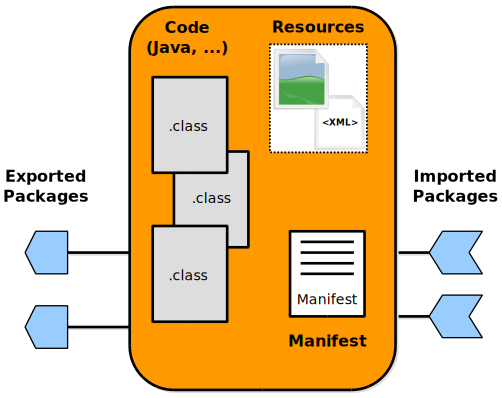
\includegraphics[height=.8\textheight]{../imgs/bundle}
\end{frame}

\begin{frame}{OSGi Bundle Life Cycle}
\centering

\tikzset{
    %Define standard arrow tip
    >=stealth',
    %Define style for boxes
    punkt/.style={
           rectangle,
           rounded corners,
           draw=black, very thick,
           fill=yellow!30,
           text width=6.5em,
           minimum height=2em,
           text centered},
    % Define arrow style
    pil/.style={
           ->,
           thick,
           shorten <=2pt,
           shorten >=2pt,}
}

\begin{tikzpicture}[node distance=2.5em, auto]
\node[circle, draw, very thick, fill=yellow!30] (init) {};
\node[punkt, below=of init] (installed) {INSTALLED};
\node[punkt, below=of installed] (resolved) {RESOLVED};
\node[punkt, below=of resolved] (uninstalled) {UNINSTALLED};
\node[punkt, right=of installed] (starting) {STARTING};
\node[punkt, right=of resolved] (active) {ACTIVE};
\node[punkt, right=of uninstalled] (stopping) {STOPPING};
\node[circle, draw, very thick, fill=black, below=of uninstalled] (final) {};

\draw[pil] (init.south) to node[auto, swap] {Install} (installed.north);
\draw[pil, <->] (installed.south) to node[auto, swap] {Resolve} (resolved.north);
\draw[pil] (resolved.east) to node[auto] {Start} (starting.west);
\draw[pil] (starting.south) to node[auto] {} (active.north);
\draw[pil] (active.south) to node[auto] {Stop} (stopping.north);
\draw[pil] (stopping.west) to node[auto] {} (resolved.east);
\draw[pil] (resolved.south) to node[auto, swap] {Uninstall} (uninstalled.north);
\draw[pil, bend right=35] (installed.west) to node[auto, swap] {Uninstall} (uninstalled.west);
\draw[pil] (uninstalled.south) to node[auto] {} (final.north);
\end{tikzpicture}
\end{frame}